\documentclass[12pt]{article}

%%%%%%%%%%%%%%%%%%%%%%%%%%%%%%%%%%%%%%%%%%%%%%%%%%%%%%%%%%%%%%%%%%%%%%%%%%%%%%%%
%                           Package preset for homework
%%%%%%%%%%%%%%%%%%%%%%%%%%%%%%%%%%%%%%%%%%%%%%%%%%%%%%%%%%%%%%%%%%%%%%%%%%%%%%%%
% Miscellaneous
\usepackage[margin=1in]{geometry}
\usepackage[utf8]{inputenc}
\usepackage{indentfirst}
\usepackage{blindtext}
\usepackage{graphicx}
\usepackage{xr-hyper}
\usepackage{hyperref}
\usepackage{enumitem}
\usepackage{color}
\usepackage{float}
% Math
\usepackage{latexsym}
\usepackage{amsfonts}
\usepackage{amssymb}
\usepackage{amsmath}
\usepackage{commath}
\usepackage{amsthm}
\usepackage{bbold}
\usepackage{bm}
% Physics
\usepackage{physics}
\usepackage{siunitx}
% Code typesetting
\usepackage{listings}
% Citation
\usepackage[authoryear]{natbib}
\usepackage{appendix}
\usepackage[capitalize]{cleveref}
% Title & name
\title{Homework}
\author{Tien Vo}
\date{\today}


%%%%%%%%%%%%%%%%%%%%%%%%%%%%%%%%%%%%%%%%%%%%%%%%%%%%%%%%%%%%%%%%%%%%%%%%%%%%%%%%
%                   User-defined commands and environments
%%%%%%%%%%%%%%%%%%%%%%%%%%%%%%%%%%%%%%%%%%%%%%%%%%%%%%%%%%%%%%%%%%%%%%%%%%%%%%%%
%%% Misc
\sisetup{load-configurations=abbreviations}
\newcommand{\due}[1]{\date{Due: #1}}
\newcommand{\hint}{\textit{Hint}}
\let\oldt\t
\renewcommand{\t}[1]{\text{#1}}

%%% Bold sets & abbrv
\newcommand{\N}{\mathbb{N}}
\newcommand{\Z}{\mathbb{Z}}
\newcommand{\R}{\mathbb{R}}
\newcommand{\Q}{\mathbb{Q}}
\let\oldP\P
\renewcommand{\P}{\mathbb{P}}
\newcommand{\LL}{\mathcal{L}}
\newcommand{\FF}{\mathcal{F}}
\newcommand{\HH}{\mathcal{H}}
\newcommand{\NN}{\mathcal{N}}
\newcommand{\ZZ}{\mathcal{Z}}
\newcommand{\RN}[1]{\textup{\uppercase\expandafter{\romannumeral#1}}}
\newcommand{\ua}{\uparrow}
\newcommand{\da}{\downarrow}

%%% Unit vectors
\newcommand{\xhat}{\vb{\hat{x}}}
\newcommand{\yhat}{\vb{\hat{y}}}
\newcommand{\zhat}{\vb{\hat{z}}}
\newcommand{\nhat}{\vb{\hat{n}}}
\newcommand{\rhat}{\vb{\hat{r}}}
\newcommand{\phihat}{\bm{\hat{\phi}}}
\newcommand{\thetahat}{\bm{\hat{\theta}}}

%%% Other math stuff
\providecommand{\units}[1]{\,\ensuremath{\mathrm{#1}}\xspace}
% Set new style for problem
\newtheoremstyle{problemstyle}  % <name>
        {10pt}                   % <space above>
        {10pt}                   % <space below>
        {\normalfont}           % <body font>
        {}                      % <indent amount}
        {\bfseries\itshape}     % <theorem head font>
        {\normalfont\bfseries:} % <punctuation after theorem head>
        {.5em}                  % <space after theorem head>
        {}                      % <theorem head spec (can be left empty, 
                                % meaning `normal')>

% Set problem environment
\theoremstyle{problemstyle}
\newtheorem{problemenv}{Problem}[section]
\newenvironment{problem}[1]{%
  \renewcommand\theproblemenv{#1}%
  \problemenv
}{\endproblemenv}
% Set lemma environment
\newenvironment{lemma}[2][Lemma]{\begin{trivlist}
\item[\hskip \labelsep {\bfseries #1}\hskip \labelsep {\bfseries #2.}]}{\end{trivlist}}
% Set solution environment
\newenvironment{solution}{
    \begin{proof}[Solution]$ $\par\nobreak\ignorespaces
}{\end{proof}}
\numberwithin{equation}{problemenv}

%%% Page format
\setlength{\parindent}{0.5cm}
\setlength{\oddsidemargin}{0in}
\setlength{\textwidth}{6.5in}
\setlength{\textheight}{8.8in}
\setlength{\topmargin}{0in}
\setlength{\headheight}{18pt}

%%% Code environments
\definecolor{dkgreen}{rgb}{0,0.6,0}
\definecolor{gray}{rgb}{0.5,0.5,0.5}
\definecolor{mauve}{rgb}{0.58,0,0.82}
\lstset{frame=tb,
  language=Python,
  aboveskip=3mm,
  belowskip=3mm,
  showstringspaces=false,
  columns=flexible,
  basicstyle={\small\ttfamily},
  numbers=none,
  numberstyle=\tiny\color{gray},
  keywordstyle=\color{blue},
  commentstyle=\color{dkgreen},
  stringstyle=\color{mauve},
  breaklines=true,
  breakatwhitespace=true,
  tabsize=4
}
\lstset{
  language=Mathematica,
  numbers=left,
  numberstyle=\tiny\color{gray},
  numbersep=5pt,
  breaklines=true,
  captionpos={t},
  frame={lines},
  rulecolor=\color{black},
  framerule=0.5pt,
  columns=flexible,
  tabsize=2
}


\title{Homework 3: Phys 5210 (Fall 2021)}

\begin{document}
   
\maketitle

%%%%%%%%%%%%%%%%%%%%%%%%%%%%%%%%%%%%%%%%%%%%%%%%%%%%%%%%%%%%%%%%%%%%%%%%%%%%%%%%
\begin{problem}{1}
    A mass $M$ is connected by a massless rod of length $l$ to a bead of mass
    $m$ which can slide along a horizontal railing without friction, as shown in
    the figure. The mass $M$ and the bead undergo motion where their center of
    mass does not move in the horizontal direction, with gravity pulling on $M$
    downwards. Find the trajectory which the mass $M$ follows in its motion.
    \begin{figure}[h]
        \centering
        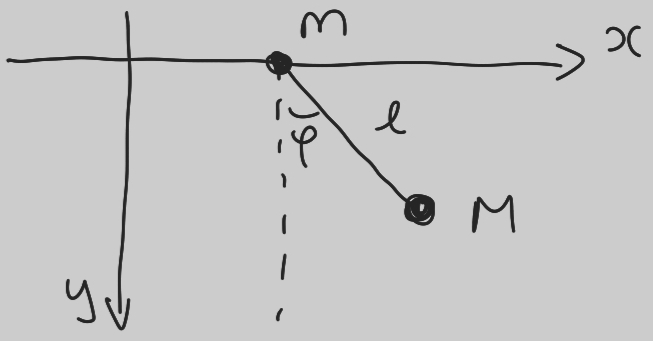
\includegraphics[width=0.5\textwidth]{hw3_p1.jpg}
    \end{figure}
\begin{solution}
    Define the coordinates as drawn in the figure. The position
    $\vb{r}_m=(x_m,y_m)$ of the bead and $\vb{r}_M=(x_M,y_M)$ of the mass $M$ 
    are as follows
    \begin{align}
        x_m&=x & x_M&=x+l\sin\varphi\notag\\
        y_m&=0 & y_M&=-l\cos\varphi
    \end{align}
    By definition, the position of the center of mass is thus
    \begin{align}
        \vb{r}_{COM}
        &=\frac{m}{m+M}\vb{r}_m+\frac{M}{m+M}\vb{r}_M\notag\\
        &=\qty(x+\frac{M}{m+M}l\sin\varphi)\xhat
        -\frac{M}{m+M}l\cos\varphi\yhat\notag\\
        &=\qty(x_M+\frac{m}{m+M}l\sin\varphi)\xhat
        -\frac{M}{m+M}l\cos\varphi\yhat
    \end{align}
    Requiring that $\dot{x}_{COM}=0$ leads to the differential equation
    \begin{equation}
        \frac{dx_M}{dt}=-\frac{m}{m+M}l\cos\varphi\frac{d\varphi}{dt} 
    \end{equation}
    Integrating both sides, we can write $x_M=-ml\sin\varphi/(m+M)$. Now, we
    have
    \begin{equation}
        x_M^2=\qty(\frac{m}{m+M})^2l^2\sin^2\varphi
        \qquad\text{and}\qquad
        y_M^2=l^2\cos^2\varphi
    \end{equation}
    Thus, the position of the mass $M$ follows
    \begin{equation}
        \qty(1+\frac{M}{m})^2x_M^2+y_M^2=l^2 
    \end{equation}
    This is an elliptical trajectory. The dependence of its ellipticity on the
    mass ratio $M/m$ is demonstrated in the figure below. If the bead is much
    more massive than the mass (magenta curve), then the bead is very inertial
    and will not accelerate too much. In this case, the mass has a circular
    trajectory, as expected of a single pendulum. The ellipticity increases as
    the bead becomes less massive compared to the mass. In the other limit where
    the mass is much more massive than the bead (green curve), then the center
    of mass is much closer to the mass. Since we require that the motion of the
    center of mass is only vertical, the mass should also roughly follow this
    trajectory.
    \begin{figure}[h]
        \centering
        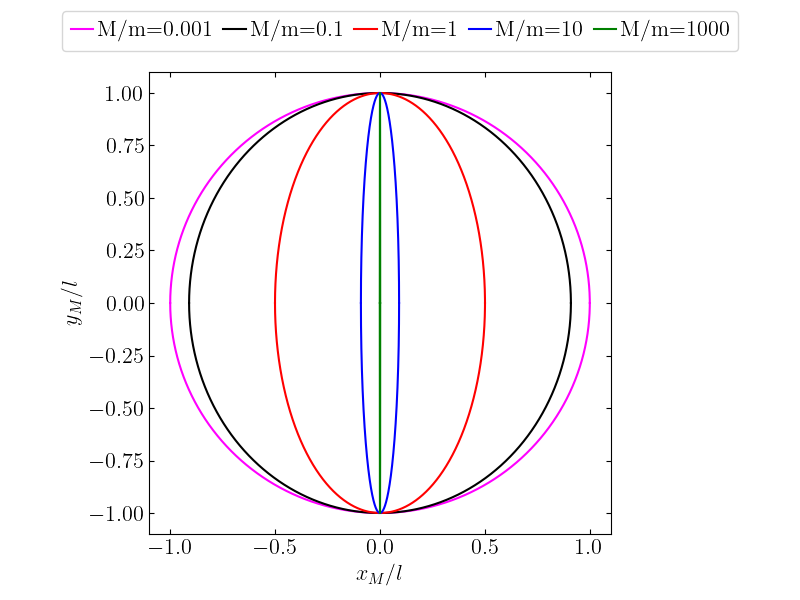
\includegraphics[width=0.8\textwidth]{p1.png}
    \end{figure}
\end{solution}
\end{problem}
%%%%%%%%%%%%%%%%%%%%%%%%%%%%%%%%%%%%%%%%%%%%%%%%%%%%%%%%%%%%%%%%%%%%%%%%%%%%%%%%
\begin{problem}{2}
    Planets in their motion around the sun are supposed to follow elliptical
    trajectories. However, in practice their trajectories deviate from perfect
    ellipses. Some of that deviation can be explained if gravitational pull of
    other planets is taken into account. It has been known since the 19th
    century that the shift of the perihelion of Mercury (the point where it is
    the closest to the sun) cannot be explained merely by gravity of other
    planets. We now know that this shift is due to the effects of general
    relativity. If we did not know about it, we could perhaps hypothesize the
    existence of a correction to the Newtonian gravity which perhaps could be
    written as
    \begin{equation}
        U(r)=-\frac{\alpha}{r}+\frac\beta{r^2} 
    \end{equation}
    where $\alpha=GMm$, $M$ is the solar mass and $m$ is the mass of a planet,
    and $\beta$ is some constant. Find the shift of the point closest to the sun
    after the planet completes one full revolution about the Sun, assuming that
    $\beta/R\ll\alpha$ where $R$ is the typical distance between the planet and
    the sun, by Taylor expanding in powers of $\beta$ and keeping the lowest
    term.
    
    \textit{Hint}: In this kind of problems, we have to deal with integrals of
    the (rough) form
    \begin{equation}
        \int_{r_{\min}}^{r_{\max}}\frac{dr}{\sqrt{E-U(r)-l^2/2\mu r^2}} 
    \end{equation}
    Direct Taylor expansion of this in powers of $\beta$ is problematic because
    it leads to integrals of the form
    \begin{equation}
        \int_{r_{\min}}^{r_{\max}}\frac{\beta dr}{r^2(E+\alpha/r-l^2/2\mu
        r^2)^{3/2}}
    \end{equation}
    This integral would be divergent as $r$ approaches the limits of integration
    where the expression in the round bracket vanishes. Instead, rewrite this
    integral as
    \begin{equation}\label{p2:hint}
        -\frac{2\mu}{l}\frac{\partial}{\partial l}\int_{r_{\min}}^{r_{\max}}dr
        r^2\sqrt{E-U(r)-\frac{l^2}{2\mu r^2}} 
    \end{equation}
    and only then expand in powers of $\beta$.
    \begin{solution}
        The energy of a two-body orbit system is
        \begin{equation}\label{p2:E}
            E=\frac{\mu\dot{r}^2}{2}+U(r)+\frac{l^2}{2\mu r^2} 
        \end{equation}
        where $\mu=mM/(m+M)$ is the reduced mass of the system, and $r$ is the
        relative distance between the two bodies. As discussed in class,
        the angular momentum $l=\mu\dot\varphi r^2$ is conserved. From
        \eqref{p2:E}, we can write the differential equation
        \begin{equation}
            \frac{dr}{dt}=\sqrt{\frac2\mu}\qty(E-U(r)-\frac{l^2}{2\mu
            r^2})^{1/2} 
        \end{equation}
        By using $dt=d\varphi \mu r^2/l$, we can write
        \begin{align}
            d\varphi
            &=\frac{l}{\sqrt{2\mu}}r^{-2}\qty(E-\frac{l^2}{2\mu
            r^2}-U(r))^{-1/2}dr\notag\\
            &=-\sqrt{2\mu}\frac{\partial}{\partial l}\qty(E-\frac{l^2}{2\mu
            r^2}-U(r))^{1/2}dr\tag{from \eqref{p2:hint}}\\
            &\approx-\sqrt{2\mu}\frac{\partial}{\partial
            l}\qty[
            \sqrt{E-\frac{l^2}{2\mu r^2}+\frac{\alpha}{r}}
            -\frac{\beta}{2 r^2}\qty(E-\frac{l^2}{2\mu
            r^2}+\frac{\alpha}{r})^{-1/2}
            ]dr\notag\\
            &=\qty{r^{-2}\qty(-\frac1{r^2}+\frac{2\mu\alpha}{l^2}\frac1r
                +\frac{2\mu E}{l^2})^{-1/2}
            +\mu\beta\frac{\partial}{\partial l}\qty[\frac1l
                r^{-2}\qty(-\frac1{r^2}+\frac{2\mu\alpha}{l^2}\frac1r
                +\frac{2\mu E}{l^2})^{-1/2}
            ]
            }dr
        \end{align}
        Integrating both sides, we get
        \begin{equation}\label{p2:dphi}
            \varphi=I+\mu\beta\frac{\partial}{\partial l}\qty(\frac{I}{l}) 
        \end{equation}
        where
        \begin{equation}
            I=\int
                r^{-2}\qty(-\frac1{r^2}+\frac{2\mu\alpha}{l^2}\frac1r+\frac{2\mu
                E}{l^2})^{-1/2}dr
        \end{equation}
        We have solved this integral in class. By a change of variables $r=1/x$,
        we can write
        \begin{equation}
            I=-\int dx\qty(-x^2+\frac{2\mu\alpha}{l^2}x+\frac{2\mu
            E}{l^2})^{-1/2}
            =-\int dx\qty[-(x-x_+)(x-x_-)]^{-1/2}
        \end{equation}
        where
        \begin{equation}
            x_\pm=\frac{\mu\alpha}{l^2}
                \pm\sqrt{\frac{\mu^2\alpha^2}{l^4}+\frac{2\mu E}{l^2}} 
        \end{equation}
        By another change of variables $x=(x_++x_-)/2+(x_+-x_-)y/2$, the
        integral $I$ turns into
        \begin{equation}
            I=-\int\frac{dy}{\sqrt{1-y^2}}=-\sin^{-1}(y)
        \end{equation}
        Since $x=1/r$, $x_+$ correponds to the point at the closest approach and
        $x_-$ corresponds to that at the furthest approach. From
        \eqref{p2:dphi}, integrating $I$ from $x_+$ to $x_-$ results in the
        angular difference of half of the system orbit, which leads to $I=\pi$.
        Here, note that $I$ describes the angular evolution of the unperturbed
        system ($\beta=0$). Without the perturbation, a full revolution of this
        orbital system corresponds to an angular sweep of $\varphi=0\to2\pi$.
        
        The second term in \eqref{p2:dphi} describes the first order
        perturbation of this angular evolution when $\beta\neq0$. Thus, the
        phase shift of the point of the closest approach in half an orbital 
        period is
        \begin{equation}
            \Delta\varphi_{\text{half}}
            =\varphi-\pi=\mu\beta\pi\frac{\partial}{\partial
            l}\qty(\frac1l)=-\pi\frac{\mu\beta}{l^2}
        \end{equation}
        It then follows from symmetry of the orbital trajectory that the shift 
        in one period is
        $\Delta\varphi_{\text{full period}}=-2\pi(\mu\beta/l^2)$.
    \end{solution}
\end{problem}
%%%%%%%%%%%%%%%%%%%%%%%%%%%%%%%%%%%%%%%%%%%%%%%%%%%%%%%%%%%%%%%%%%%%%%%%%%%%%%%%
\end{document}
